\setcounter{page}{1}
\section*{Zielsetzung}
In dem Versuch V47 wird die Molwärme von Kupfer $\ce{Cu}$ bestimmt.
Der Begriff Molwärme wird hierbei als Synonym für die \emph{molare Wärmekapazität} verwendet.
Diese gibt die Wärmemenge an, die benötigt wird um $\SI{1}{\mol}$ eines Stoffes
bzw. Elementes um einen $\SI{1}{\kelvin}$ zu erwärmen.

\section{Theorie}\label{sec:theorie}
Im Folgenden werden drei Methodiken zur Bestimmung der Molwärme erläutert.
Zunächst wird die Molwärme klassisch hergeleitet. Anschließend werden zwei
quantenmechanische Modelle von \emph{Einstein} und \emph{Debye}
vorgestellt. Hierfür werden die Quellen \cite{anleitungV47} und \cite[S. 215]{marx} verwendet.

Weiterhin kann die Molwärme bei unterschiedlichen Bedingungen betrachtet werden.
Wird der äußere Druck $p$ festgehalten, wird von der Wärmekapazität bei konstantem
Druck gesprochen. Aus der Thermodynamik folgt für diesen Fall der Zusammenhang:
\begin{equation}
  \label{eq:C_P}
  C\ua{p} = \left.\frac{\partial Q}{\partial T}\right|_{\map{p}}.
\end{equation}
Anstatt des Druckes $p$ kann auch das Volumen des Festkörpers $V$ festgehalten
werden. Dies definiert die Wärmekapazität bei konstantem Volumen:
\begin{equation}
  \label{eq:C_V}
  C\ua{V} = \left.\frac{\partial Q}{\partial T}\right|_{V} = \left. \frac{\partial U}{\partial T}\right|_{V}.
\end{equation}
Auf Grund der Tatsache, dass sich $C\ua{V}$ aus der inneren Energie $U$ ableiten
lässt, ist die Beschreibung über ein theoretisches Modell leichter zu realisieren.
Jedoch kann in einem Experiment kaum sichergestellt werden, dass das Volumen einer
Probe konstant bleibt. Deshalb wird meist $C_p$ gemessen und mit Hilfe
der Formel
\begin{equation}
  \label{eq: C_V}
  C\ua{p} - C\ua{V} = 9\alpha^2 \kappa V_0 T
\end{equation}
in $C_V$ umgerechnet. Die in der Gleichun \eqref{eq: C_V} auftretenden
Größen sind - der lineare Ausdehungskoeffizient $\alpha$, das Kompressionsmodul
$\kappa$ und das Molvolumen $V_0$.
\subsection{Klassische Betrachtung}
Klassisch lässt sich die mittlere freie innere Energie $\left<U\right>$ aus dem
\emph{Äquipartitionstheorem} ableiten. Dieses besagt, dass auf jeden quadratischen
Freiheitsgrad eine mittlere Energie von $\frac{1}{2}\map{k_B}T$ entfällt.
Für ein einzelnes Atom ergibt sich somit aus der kinetischen Energie $\frac{1}{2}mv_i^2$ und
dem quadratischen Potential der Gitterschwingung $\frac{1}{2}kx_i^2$:
\begin{equation}
  \label{eq:innere_Energie}
  \left<U\,\right> = \underbrace{3}_{\map{Raumrichtungen}}\map{k_B}T.
\end{equation}
Für die innere Energie pro $\si{mol}$ ergibt sich mit der Avogardokonstante
$\map{N_A}$ folglich:
\begin{equation}
  \label{eq:klassische_innere_Energie}
  \left<U\,\right> = 3\underbrace{\map{N_A} \map{k_B}}_{=\map{R}} T.
\end{equation}
Aus der Gleichung \eqref{eq:klassische_innere_Energie} lässt sich das
\emph{Dulong-Petische Gesetz} ableiten:
\begin{equation}
  \label{eq:dulong_petit}
  C\ua{V}=\left. \frac{\partial U}{\partial T}\right|_{V}=3R
\end{equation}
Nach dem Dulong-Petischen Gesetz ist die Wärmekapazität jedoch Material und
temperaturunabhängig. Im späteren Verlauf werden wir zeigen, dass das Dulong-Petische Gesetz
im Grenzfall aus den quantenmechanischen Theorien folgt.

\subsection{Quantenmechanische Betrachtung}
Die bisherige klassische Betrachtungsweise der inneren Energie hat die
Quantisierung der Gitterschwingung nicht berücksichtigt.
Gitterschwinungen lassen sich als quantenmechanische Oszillatoren vereinfacht darstellen. Für diese
sind die zugehörigen Eigenenergien gegeben durch
\begin{equation}
  \label{eq:energie_quanten_oszi}
  E_n = \hbar \omega \left(n + \frac{1}{2}\right).
\end{equation}
Über die Zustandssumme des quantenmechanischen Systems lässt sich die innere Energie
für $3N$ harmonische Oszillatoren wie folgt berechnen:
\begin{equation}
  \label{eq:innere_energie}
  \left<U\right> = -3N\frac{1}{Z}\partial_\beta Z, \quad \text{mit} \quad \beta = \frac{1}{\map{k_B}T}
\end{equation}
Hierbei ist die Zustandssumme für die obige Energie (vgl. Gleichung \eqref{eq:energie_quanten_oszi})
gegeben als
\begin{equation}
  \label{eq:Zustandsumme}
  Z = \sum_n^\infty \exp\left(-\beta\hbar\omega\left(n+\frac{1}{2}\right)\right).
\end{equation}
Wird die Zustandssumme \eqref{eq:Zustandsumme} in die Gleichung \eqref{eq:innere_energie}
eingesetzt folgt:
\begin{equation*}
  \left<U\right>= 3N  \frac{ \sum_n^\infty \hbar\omega\left( n+ \frac{1}{2} \right)\exp\left(-\beta\hbar\omega\left( n+\frac{1}{2} \right) \right) }{ \sum_n^\infty \exp\left( -\beta\hbar\omega\left( n+\frac{1}{2} \right) \right)}.
\end{equation*}
Nach einigen Umformungsschritten - nachlesbar in Quelle \cite[S. 220]{marx} - folgt für die innere Energie:
\begin{equation}
  \label{eq:innere_Energie_Quantenmechanik_diskrete}
  \left<U\right> = 3N\hbar\omega\left(\frac{1}{2} + \frac{1}{\exp\left(\hbar\omega\beta\right) -1}\right).
\end{equation}
Hierbei ist $\frac{1}{\exp\left(\hbar\omega\beta\right) -1}$ die \emph{Bose-Einstein Statistik}.

\subsubsection{Einstein-Modell}
Das von Albert Einstein im Jahre 1907 formulierte Modell nimmt eine konstante
Dispersionsrelation für alle $3N$ Eigenschwingung an:
\begin{equation}
  \label{eq:dispersion_einstein}
  \omega=\omega\ua{E}=\map{const}.
\end{equation}
Für die Wärmekapazität folgt, unter Verwendung von Gleichung \eqref{eq:innere_Energie_Quantenmechanik_diskrete}, somit:
\begin{equation}
  \label{eq:CV_einstein}
  C\ua{V}^{\map{E}}= 3N\map{k_B}\left(\frac{\Theta\ua{E}}{T}\right)^2\frac{\exp\left(\frac{\Theta\ua{E}}{T}\right)}{\left(\frac{\Theta\ua{E}}{T}-1\right)^2}, \quad \text{mit} \quad \Theta\ua{E} = \frac{\hbar\omega\ua{E}}{\map{k_B}}
\end{equation}
Wird die Approximation \eqref{eq:CV_einstein} für hohe und niedrige Temperaturen
betrachtet, folgt:
\begin{equation}
  C\ua{V}^{\map{E}}=
  \begin{cases}
     3N\map{k_B}\left(\frac{\Theta\ua{E}}{T}\right)^2 \exp\left(-\frac{\Theta\ua{E}}{T}\right), &\text{für } T\ll\Theta\ua{E}  \\
     3N\map{k_B}, & \text{für } T \gg \Theta\ua{E}
  \end{cases}
\end{equation}
Bei der Betrachtung der Anzahl der Atome pro $\si{mol}$ kann $N$ durch $\map{N_A}$
ersetzt werden und es ergibt sich das in \eqref{eq:dulong_petit} definierte
Dulong-Petische Gesetz. In der Abbildung \ref{fig: einstein_modell_plot} ist zu erkennen, wie das Einstein-Modell
experimentelle Daten beschreibt.
\begin{figure}
  \centering
  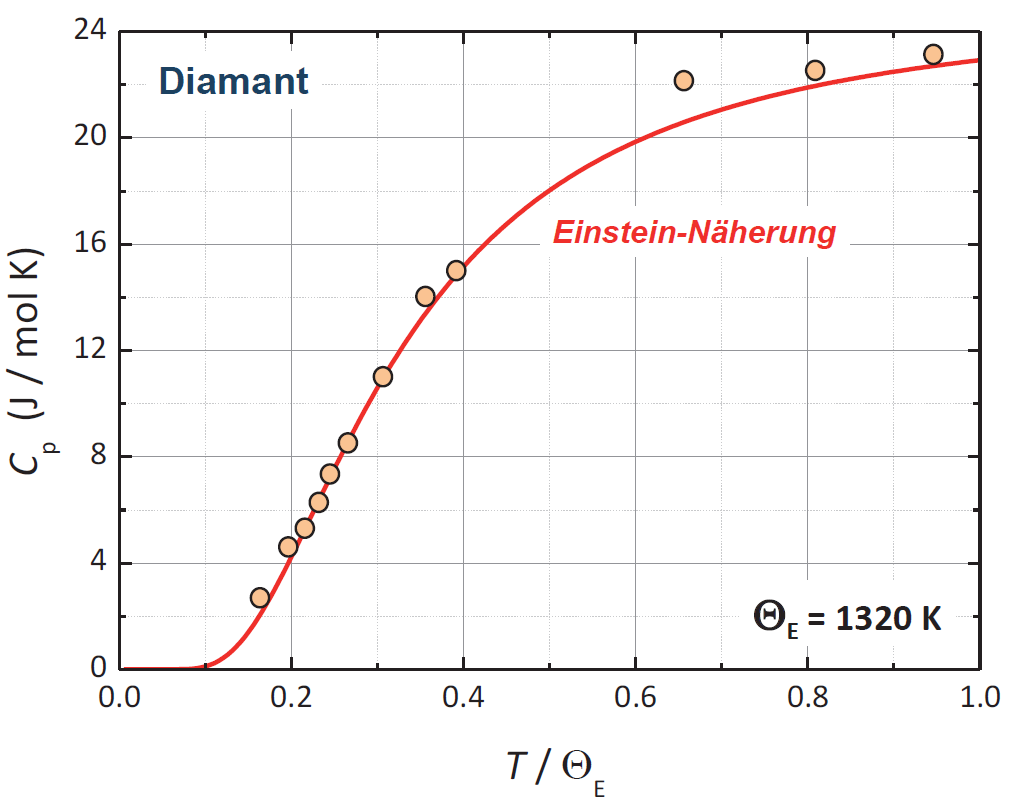
\includegraphics[width = 0.65\textwidth]{./content/images/einstein.PNG}
  \caption{Die experimentell Bestimmte molare Wärmekapazität von Diamant. Zusätzlich ist die durch das Einstein-Modell
  gegebene theoretische Beschreibung mit eigezeichnet \cite[S. 225]{marx}.}
  \label{fig: einstein_modell_plot}
\end{figure}
Das Einstein-Modell eignet sich gut, wenn optische Phononen dominieren oder eine
flache Dispersionsrelation vorliegen (vgl. Abbildung \ref{fig: dispersions_relation}).
\begin{figure}
  \centering
  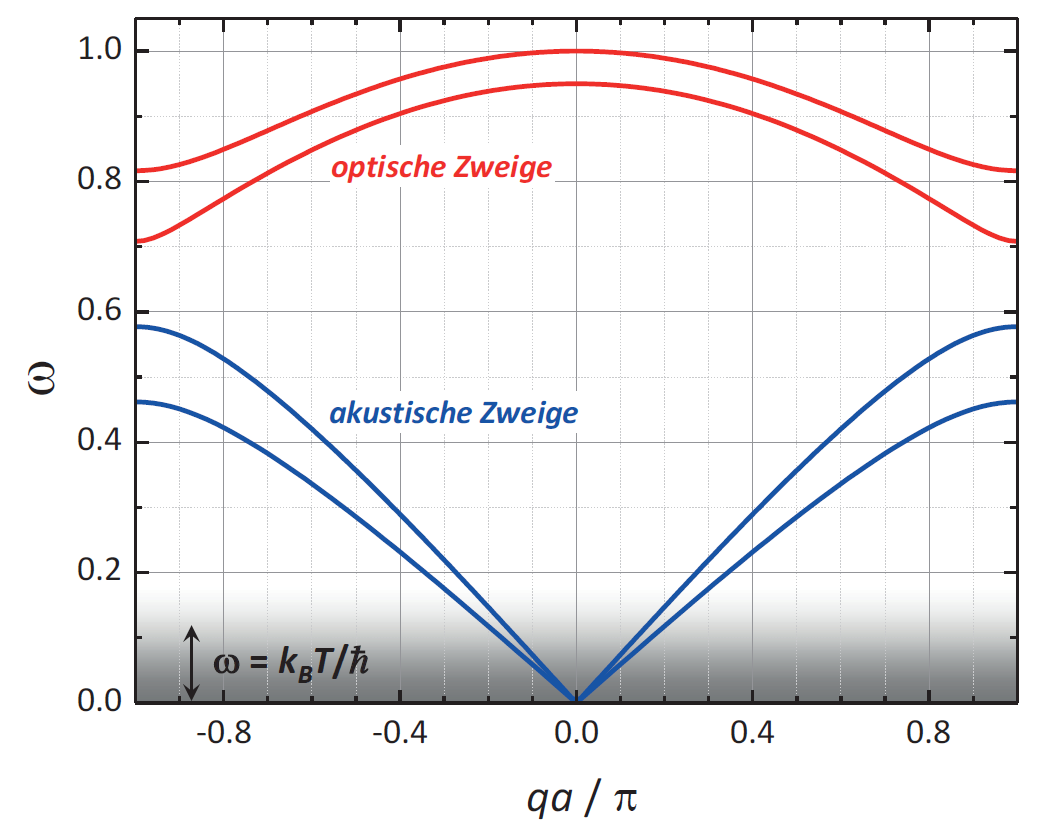
\includegraphics[width = 0.65\textwidth]{./content/images/optische_akustische.PNG}
  \caption{Schematische Darstellung von optischen und akustischen Dispersionszweigen \cite[S. 223]{marx}.}
  \label{fig: dispersions_relation}
\end{figure}
Zusätzlich ist in der Abbildung \ref{fig: dispersions_relation} deutlich zu erkennen,
dass akustische Phononen um Null eine annähernd lineare Dispersionsrelation aufweist.
Dies ist die Motivation für das zweite quantenmechanische Modell, das
Debye-Modell.

\subsubsection{Debye-Modell}
Im Debye-Modell wird eine lineare Dispersionsrelation angenommen:
\begin{equation*}
   \omega = \hbar \be{\vec{k}}.
\end{equation*}
Hierdurch muss die Summation in Gleichung \eqref{eq:Zustandsumme} durch eine
Integration ersetzt werden. Die Integrationsgrenzen werden so gewählt, dass über die
erste Brillouin-Zone integriert wird. Hierbei wird die erste Brillouin-Zone
weiter als Kugel mit dem Radius $k\ua{D}$ genährt. Der Betrag des Debye-Wellenvektors
$k\ua{D}$ kann über die Zustandsvolumen bestimmt werden. Ein Zustand besitzt im $k$-Raum
ein Volumen von $V=\frac{8\pi^3}{L^3}$. Ingesamt betrachten wir $N$ Zustände pro
Dispersionszweig, daraus ergibt sich:
\begin{align*}
  N\left(\frac{2\pi}{L}\right)^3 &= \frac{4}{3}\pi k^3\ua{D} \\
  \Leftrightarrow \quad k\ua{D}&=\left(6\pi^2 \frac{N}{V}\right)^{\frac{1}{3}}, \quad \text{mit} \quad L^3 = \left(\frac{2\pi}{V}\right)
\end{align*}
Für eine lineare Dispersion folgt für die Zustandsdichte:
\begin{equation}
  \label{eq:Zustandsichte_debye}
D(\omega)_i = \frac{V}{\left(2\pi\right)^3} \int_{\omega=\map{const}} \frac{\map{d}S\ua{k}}{\be{\nabla_k \omega(\vec{k})}}= \frac{V}{2\pi^2}\frac{\omega^2}{\nu_i^3}
\end{equation}
Hierbei ist das in Gleichung \eqref{eq:Zustandsichte_debye} auftretende Integral
über der Kugel mit dem Radius $\omega=\map{const}$ und $\nu_i$ die Schallgeschwindigkeit
des $i$-ten Dispersionszweig. In diesem Fall werden zwei transversale und ein optischer
Ast betrachtet:
\begin{equation}
  \label{eq:Zustandsdichte_all_togther}
  D(\omega) = \frac{V \omega^2}{2\pi^2} \left(\frac{1}{\nu^3\ua{L}} + \frac{2}{\nu^3\ua{T}}\right)
\end{equation}
Nun wird ausgehend von dem Debye-Wellenvektor die Debye-Frequenz $\omega\ua{D}$ eingeführt:
\begin{equation}
  \label{eq:Debye_freuqenz}
  \omega\ua{D}^3 = \frac{18 \pi^2 N}{V}\left(\frac{1}{\nu^3\ua{L}} + \frac{2}{\nu^3\ua{T}}\right)^{-1}=\frac{6\pi^2\nu^3N}{V}.
\end{equation}
Hierbei wurde eine Mittelung über alle Schallgeschwindigkeiten $\nu^3$ durchgeführt:
\begin{equation*}
  \nu^3= \frac{1}{3}\left(\frac{1}{\nu^3\ua{L}} + \frac{2}{\nu^3\ua{T}}\right)^{-1}.
\end{equation*}
Wird die Gleichung \eqref{eq:Debye_freuqenz} in Formel \eqref{eq:Zustandsdichte_all_togther}
eingesetzt ergibt sich:
\begin{equation}
  \label{eq:Zustandsdichte_Debye}
  D(\omega)= \frac{9N\omega^2}{\omega\ua{D}^3}.
\end{equation}
Damit können wir die Wärmekapazität definieren als:
\begin{equation}
  \label{eq:CVD_ohne_x}
  C^{\map{D}}\ua{V}=\frac{9N\hbar}{\omega_D}\frac{\partial}{\partial T}\int^{\omega_D}{0}\frac{\omega^3}{\exp\left(\hbar\omega\beta\right)-1} \map{d}\omega.
\end{equation}
Nach der Durchführung der Ableitung und Substitution mit $x=\hbar\omega\beta$
folgt für die spezifische Wärmekapazität:
\begin{equation}
  \label{eq:CV_debye}
  C^{\map{D}}\ua{V}=9N\map{k_B}\left(\frac{T}{\Theta_D}\right)^3\int^{\Theta_D/T}_{0} \frac{x^4\exp(x)}{(\exp(x)-1)^2}\map{d}x.
\end{equation}
Hierbei wurde zusätzlich die \emph{Debye-Temperatur} eingeführt als
\begin{equation}
  \label{eq:Debye_Temp}
  \Theta_D = \frac{\hbar\omega_D}{\map{k_B}}.
\end{equation}
In Abbildung \ref{fig: CVD_plot} ist Formel \eqref{eq:CV_debye} grafisch dargestellt.
\begin{figure}
  \centering
  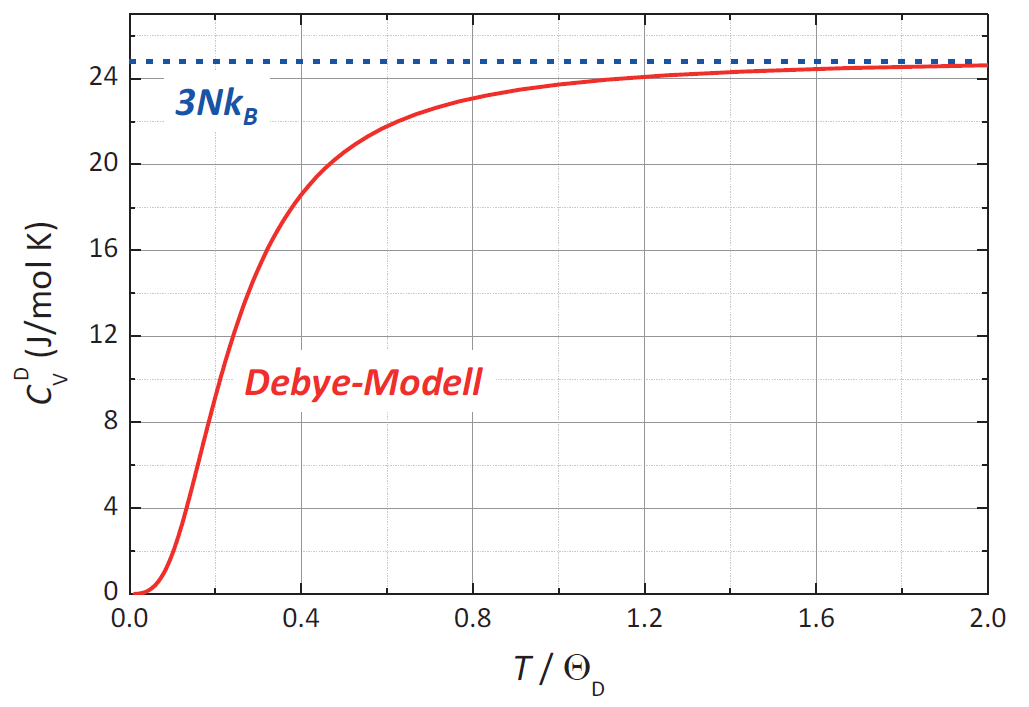
\includegraphics[width = 0.65\textwidth]{./content/images/C_V_debye.PNG}
  \caption{Schematische Darstellung der Debye-Wärmekapazität $C^{\map{D}}\ua{V}$ (vgl. Gleichung \eqref{eq:CV_debye})  \cite[S. 228]{marx}.}
  \label{fig: CVD_plot}
\end{figure}
Für hohe und tiefe Temperaturen ergibt sich approximativ:
\begin{equation}
  C\ua{V}^{D}=
  \begin{cases}
    \frac{12\pi^4}{5}N\map{k_B}\left(\frac{T^3}{\Theta_D}\right)^3, &\text{für } T\ll\Theta\ua{D}  \\
     3N\map{k_B}, & \text{für } T \gg \Theta\ua{D}.
  \end{cases}
\end{equation}
Damit folgt aus dem Debye-Modell derselbe hochtemperatur Limes, wie beim Einstein-Modell.
Die Debye-Temperatur kann somit als Maß dafür verwendet werden, ob eine klassische
oder quantenmechanische Beschreibung der Wärmekapazität einer Probe benötigt wird.
